\section{Contrastes de hipótesis}
\subsection{Introducción}
Basándonos en una muestra, queremos decidir entre dos opciones o hipótesis acerca de la distribución de interés en la población.

Las hipótesis pueden verter sobre
\begin{itemize}[label=\textbullet]
    \item La forma de la distribución: ¿Es una Poisson? ¿Es una Normal? \lb{Contrastes no paramétricos}.
    \item Los paramétricos de la distribución, si suponemos dada la familia paramétrica. \lb{Contrastes paramétricos}.
    \item Si consideramos dos variables, ¿existe una relación de dependencia? \lb{Contrastes no paramétricos}.
\end{itemize}
\subsection{Constrastes de hipótesis paramétricos}
\subsubsection{Elementos principales}
\begin{tcolorbox}[colback=red!5!white, colframe=red!75!black, title=\textbf{Idea básica}]
Un \textbf{test de hipótesis} es una regla que nos lleva a decidir si lo observado en la muestra es compatible con una hipótesis planteada sobre los parámetros del modelo.
\end{tcolorbox}
\begin{tcolorbox}[colback=blue!5!white, colframe=blue!75!black, title=\textbf{Ejemplo}]
Un nuevo medicamento pretende mejorar un medicamento del mercado, que tiene probabilidad $\theta_0=0.7$ de curar un paciente.
\begin{itemize}[label=\textbullet]
    \item Planteamos $X\sim \mathrm{Bernoulli}(\theta),X=1\longleftrightarrow$ el paciente se cura con el medicamento nuevo.
    \item Lanzamos el nuevo medicamento si $\theta>\theta_0+0.15$, es decir, que debemos decidir entre \[
    \begin{array}{l}
        H_0:\theta\le \theta_0+0.15\\
        H_1:\theta>\theta_0+0.15
    \end{array}
    \] 
\item Consideramos una m.a.s. de tamaño 100, el estadístico $T(X_1,\dots,X_{100})=\sum_{i=1}^{100} X_i$, resumen de la información muestral.
\item Posible test:
    \begin{itemize}[label=\textrightarrow]
        \item Aceptamos $H_0$ si $\sum_{i=1}^{100} X_i\le 85$.
        \item Rechazamos $H_0$ si $\sum_{i=1}^{100} X_i>85$.
    \end{itemize}
\end{itemize}
\end{tcolorbox}
Si queremos ser más conservadores: aceptamos $H_0$ si $\sum_{i=1}^{100}X_i\le 90 $, y rechazamos $H_0$ si $\sum_{i=1}^{100} X_i>90$.
\begin{tcolorbox}[colback=blue!5!white, colframe=blue!75!black, title=\textbf{Podemos cometer dos tipos de errores:}]
\begin{itemize}[label=\textbullet]
    \item Rechazar una hipótesis verdadera.
    \item Aceptar una hipótesis falsa.
\end{itemize}
\end{tcolorbox}
\subsubsection{Formulación general del contraste de hipótesis}
\begin{itemize}[label=\color{red}\textbullet, leftmargin=*]
    \item \lb{Contexto}
        \begin{itemize}[label=\textbullet]
            \item $X\sim F(x,\theta)$, con $\theta\in \Theta\subseteq \R^p$.
            \item $\mathbf{X}=(X_1,X_2,\dots,X_n)$ una m.a.s. de $X$.
            \item  $\Theta_0$ y $\Theta_1$ dos subconjuntos del espacio paramétrico $\Theta$ tales que:  $\Theta=\Theta_0\cup \Theta_1$ y $\Theta_0\cap \Theta_1=\varnothing$
        \end{itemize}
    \item \lb{Definición}

        Un \lb{test} o \lb{contraste} es una regla basada en $\mathbf{X}$ para decidir entre las dos hipótesis: \[
        H_0:\theta\in \Theta_0
        \]frente a \[
        H_1:\theta\in \Theta_1.
        \]    
\end{itemize}
\begin{tcolorbox}[colback=olive!5!white, colframe=olive!75!black, title=\textbf{Llamamos}]
\begin{itemize}[label=\textbullet]
    \item $H_0$: hipótesis nula.
    \item $H_1$: hipótesis alternativa.
\end{itemize}
\end{tcolorbox}
\begin{tcolorbox}[colback=blue!5!white, colframe=blue!75!black, title=\textbf{Definición}]
Se llama \lb{test (no aleatorizado)}  a una función $\delta:\mathrm{sop}(\mathbf{X})\to \{0,1\} $ tal que:
\begin{itemize}[label=\textbullet]
    \item si $\delta(\mathbf{x})=0$ se acepta la hipótesis nula $H_0$.
    \item si $\delta(\mathbf{x})=1$ se rechaza la hipótesis $H_0$.
\end{itemize}
\end{tcolorbox}
\begin{tcolorbox}[colback=blue!5!white, colframe=blue!75!black, title=\textbf{Notación}]
\begin{itemize}[label=\textbullet]
    \item $\mathrm{sop}(\mathbf{X})$ es el soporte de $\mathbf{X}$, que es el conjunto donde $f(x)$, la función puntual de probabilidad (caso discreto) o la funcón densidad (caso continuo) de  $X$ es $>0$.
    \item Denotaremos por  $T$ el conjunto de tests definidos sobre el $\mathrm{sop}(\mathbf{X})$.
\end{itemize}
\end{tcolorbox}
Dado un test $\delta\in T$ se definen los siguientes conjuntos:
\begin{tcolorbox}[colback=blue!5!white, colframe=blue!75!black, title=\textbf{Definición}]
\begin{itemize}[label=\textbullet]
    \item \lb{Región de aceptación:} \[
            S_0=\{\mathbf{x}\in \mathrm{sop}(\mathbf{X}):\delta(\mathbf{x})=0\} .
    \]  
\item \lb{Región de rechazo:} \[
S_1=\{\mathbf{x}\in \mathrm{sop}(\mathbf{X}):\delta(\mathbf{x})=1\} .
\]  
\end{itemize}
\end{tcolorbox}
\subsubsubsection{Errores}
\begin{itemize}[label=\color{red}\textbullet, leftmargin=*]
    \item \lb{Definimos los errores asociados}
        \begin{itemize}[label=\textbullet]
            \item Error de tipo I: rechazar $H_0$ cuando es cierta.
            \item Error de tipo II: aceptar $H_0$ cuando es falsa.
        \end{itemize}
\end{itemize}
\begin{tcolorbox}[colback=blue!5!white, colframe=blue!75!black, title=\textbf{Resumen}]
\begin{center}
    \begin{tabular}{ccc}
        & $\mathbf{X}\in S_1$ & $\mathbf{X}\in S_0$ \\ \hline
        $\theta\in \Theta_0$ & Error tipo I & Correcto\\ \hline
        $\theta\in \Theta_1$ & Correcto & Error tipo II
    \end{tabular}
\end{center}
\end{tcolorbox}
Recordad, $S_0$ región de aceptación, $S_1$ región de rechazo.
\begin{itemize}[label=\color{red}\textbullet, leftmargin=*]
    \item \lb{Definimos las probabilidades asociadas, para un test $\delta$ dado,}
        \begin{itemize}[label=\textbullet]
            \item La probabilidad de cometer un error de tipo I, si el valor del parámetro es $\theta$, se denota por:  \[
            \text{Si }\theta\in \Theta_0:\quad P_{I,\delta}(\theta)=P_\theta(\mathbf{X}\in S_1).
            \] 
        \item La probabilidad de cometer un error de tipo II, si el valor del parámetro es $\theta$, se denota por:  \[
        \text{Si }\theta\in \Theta_1:\quad P_{II,\delta}(\theta)=P_\theta(\mathbf{X}\in S_0).
        \] 
        \end{itemize}
\end{itemize}
\begin{tcolorbox}[colback=blue!5!white, colframe=blue!75!black, title=\textbf{¿Qué buscamos?}]
Queremos encontrar un test $\delta$ con  $P_{I,\delta}(\theta)$ y $P_{II,\delta}(\theta)$ lo más pequeñas poisbles \lb{simultáneamente}.
\end{tcolorbox}
\subsubsection*{Ejemplo de test: control de calidad}
\begin{tcolorbox}[colback=blue!5!white, colframe=blue!75!black, title=\textbf{Contexto}]
\begin{itemize}[label=\textbullet]
    \item En la producción de un artículo electrónico, se cuida que la tensión que circula por un componente es 10mV. Hay variabilidad en la tensión conseguida en los artículos producidos, que pensamos modelizar por una Normal con desviación típica 0.05.
    \item Para controlar la calidad de los artículos producidos, se escogen al azar cada día 20 artículos y se mide su tensión.
    \item ¿Qué regla podríamos fijar que describa cuándo debe saltar una alarma si parece que la tensión se aleja de 10mV?
\end{itemize}
\end{tcolorbox}
\begin{tcolorbox}[colback=blue!5!white, colframe=blue!75!black, title=\textbf{Traducimos el contexto}]
\begin{itemize}[label=\textbullet]
    \item $X$: tensión medida en un artículo escogido al azar en la producción.  $X\sim \mathcal{N}(\mu,0.025)$.
    \item $\mathbf{X}=(X_1,X_2,\dots,X_{20})$ una m.a.s. de $X$ de tamaño $20$.
    \item Queremos controlar si  $\mu=10$.
\end{itemize}
\end{tcolorbox}
\begin{itemize}[label=\textbullet]
    \item Planteamos las hipótesis: \[
    \begin{array}{l}
        H_0:\mu=10\\
        H_1:\mu\neq 10
    \end{array}
    \]
\item Nuestra regla, es decir nuestro test $\delta$, se basará en  $\mathbf{\overline{X}}$:
    \begin{itemize}[label=\textrightarrow]
        \item si $\mathbf{\overline{X}}$ está "alejado" de 10, rechazaremos $H_0$.
        \item si $\mathbf{\overline{X}}$ está "cerca" de 10, aceptaremos $H_0$.
    \end{itemize}
\end{itemize}
\begin{tcolorbox}[colback=blue!5!white, colframe=blue!75!black, title=\textbf{Nuestra regla}]
Nos fijamos un umbral $u$,
 \begin{itemize}[label=\textbullet]
    \item si $\mathbf{\overline{X}}<10-u$ ó $\mathbf{\overline{X}}>10+u$, rechazaremos $H_0$.
    \item si $10-u\le \mathbf{\overline{X}}\le 10+u$, aceptaremos $H_0$.
    \item $\delta(\mathbf{x})=1$, si $|\mathbf{\overline{X}}-10|>u$.
    \item $\delta(\mathbf{x})=0$, si $|\mathbf{\overline{X}}-10|\le u$.
\end{itemize}
\end{tcolorbox}
\begin{tcolorbox}[colback=blue!5!white, colframe=blue!75!black, title=\textbf{Calculamos las probabilidades de error}]
Si $\mu=10$, \[
P_\mu(\text{rechazar $H_0$})=P_\mu(|\mathbf{\overline{X}}-10|>u)=2P\left( Z>\dfrac{u}{0.05 /\sqrt{20} } \right) 
\] 
Si $\mu\neq 10$, \[
P_\mu(\text{aceptar $H_0$})=P_\mu(|\mathbf{\overline{X}}-10|\le u)=P\left( \dfrac{10-u-\mu}{0.05 /\sqrt{20} }\le Z\le \dfrac{10+u-\mu}{0.05 /\sqrt{20} } \right) 
\] 
\end{tcolorbox}
Por ejemplo, si fijamos $u=0.025,P_{\mu}$

Podemos variar $u$:
 \begin{center}
    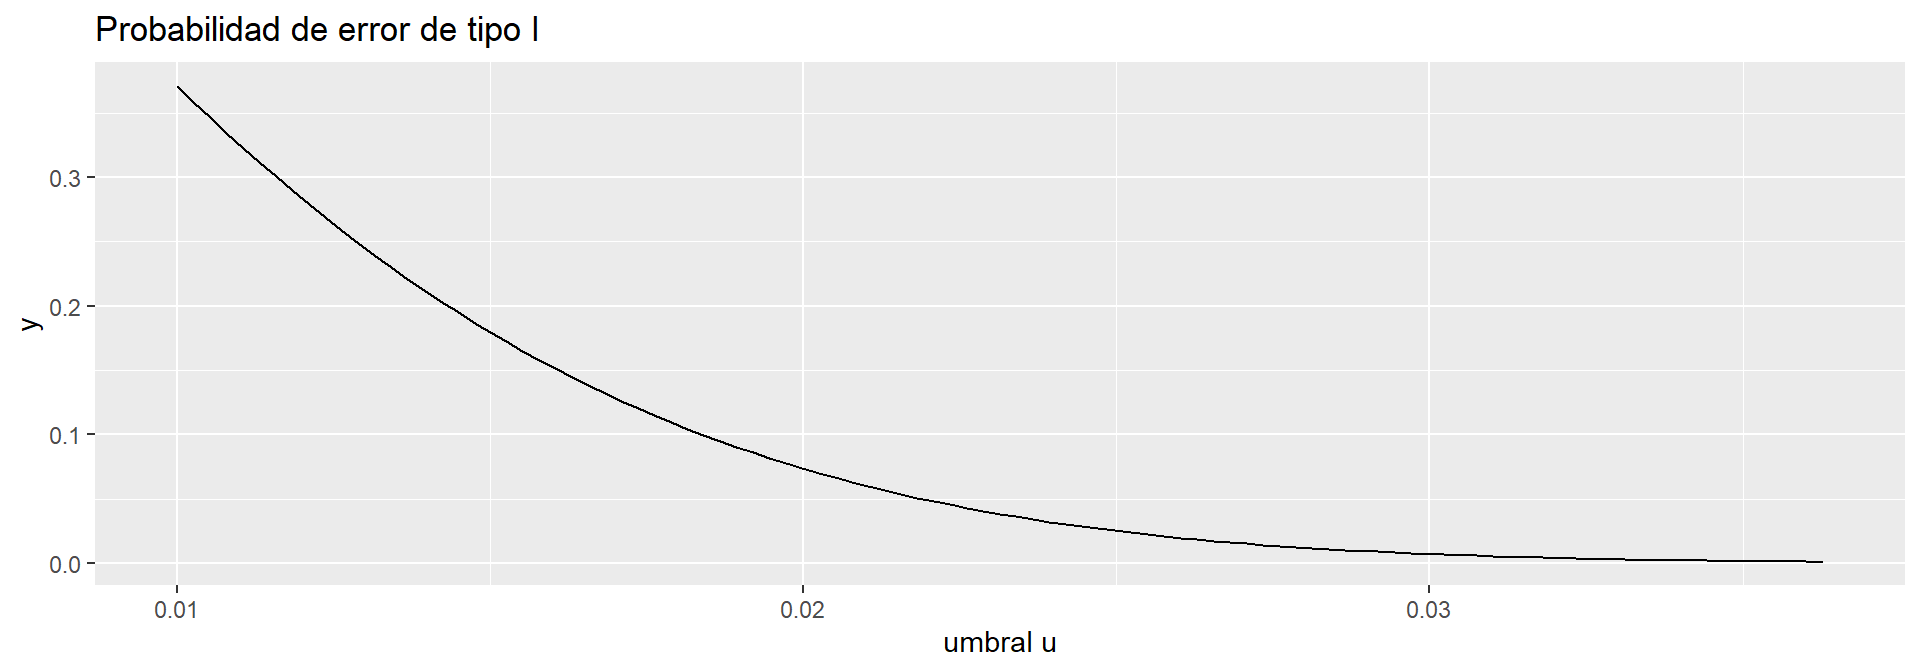
\includegraphics[width=0.7\textwidth]{Tema 4/figures/Figure 1}
\end{center}
Si fijamos $u=0.02$, tenemos una probabilidad de eror de tipo I de 0.05.

¿Qué pasa con la probabilidad de error de tipo II?
 \begin{center}
    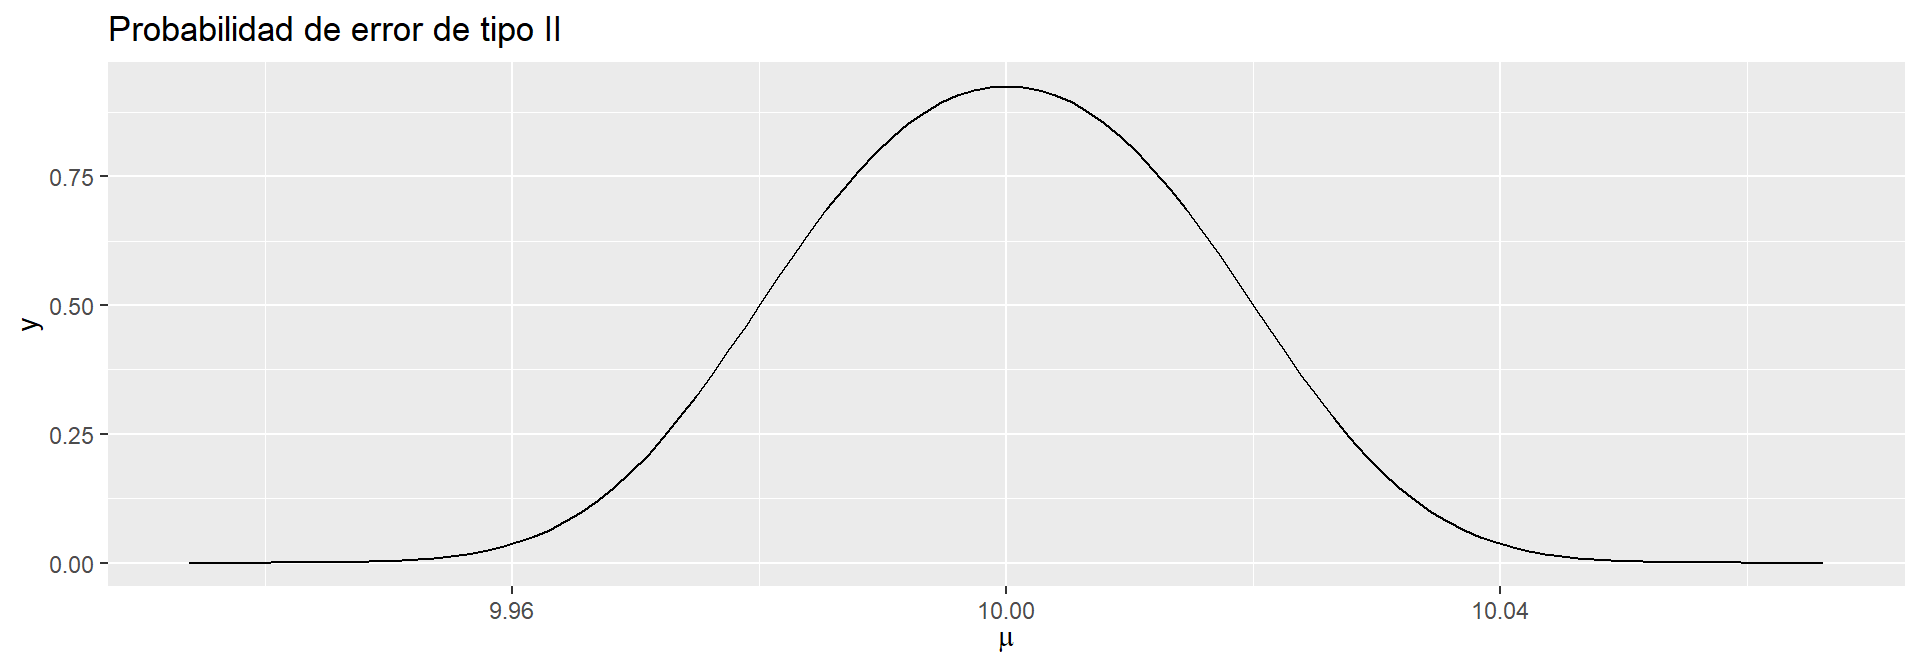
\includegraphics[width=0.7\textwidth]{Tema 4/figures/Figure 2}
\end{center}
Queremos detectar $\mu=10.05$ con una probabilidad suficiente pero a la vez, no queremos rechazar $H_0$ erróneamente con demasiada facilidad.
\begin{center}
    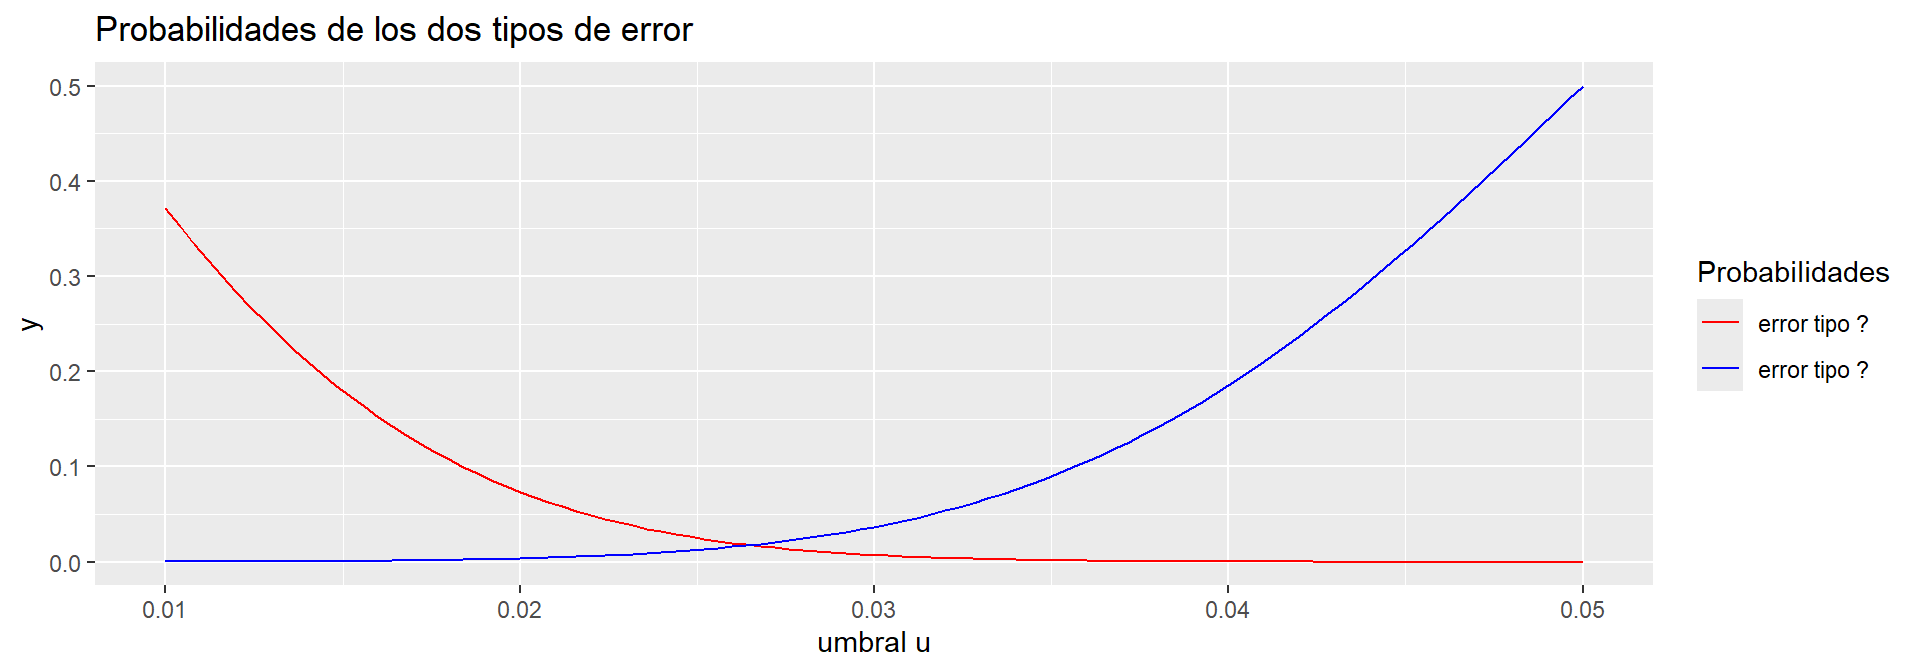
\includegraphics[width=0.7\textwidth]{Tema 4/figures/Figure 3}
\end{center}
\subsection{Métodos útiles para construir tests}
\subsubsection{Un primer procedimiento general}
\begin{tcolorbox}[colback=blue!5!white, colframe=blue!75!black, title=\textbf{Para llevar a cabo un contraste de hipótesis, podemos}]
\begin{itemize}[label=\textbullet]
    \item Formular las hipótesis $H_0$ y $H_1$.
    \item Fijarnos la probabilidad de error de tipo I, $\alpha$.
    \item Para construir nuestra regla $\delta$, escogemos el estadístico de prueba  $T(X_1,\dots,X_n)$ basado generalmente en un estimador del parámetro. Consideramos su distribución muestral suponiendo $H_0$ cierta.
    \item Determinamos la región de rechazo $S_1$, teniendo en cuenta la probabilidad de error I, es decir, \[
    P_{H_0}(T(X_1,\dots,X_n)\in S_1)=\alpha.
    \] 
\item Para nuestra muestra, calculamos $T(x_1,\dots,x_n)$ y decidimos si aceptamos o rechazamos $H_0$, según si su valor está en $S_0$ o en $S_1$.
\end{itemize}
\end{tcolorbox}
\subsection{Constraste de hipótesis para la media $\mu$}
\begin{tcolorbox}[colback=olive!5!white, colframe=olive!75!black, title=\textbf{Primer caso}]
Empezamos por considerar la construcción de un contraste para la media $\mu$ de una población Normal con varianza conocida. 
\end{tcolorbox}
\begin{tcolorbox}[colback=blue!5!white, colframe=blue!75!black, title=\textbf{Contexto}]
\begin{itemize}[label=\textbullet]
    \item Consideramos una v.a. $X$.
    \item Hemos decidido modelar:  $X\sim \mathcal{N}(\mu,\sigma^2)$.

        Tenemos fijado el valor de $\sigma$ (valor poblacional, por ejemplo gracias a datos históricos).
    \item Queremos llevar a cabo un contraste sobre $\mu$.
    \item Para ello, extraeremos una muestra de tamaño $n$ de la distribución de $X$.
\end{itemize}
\end{tcolorbox}
\subsection{Procedimiento, hipótesis bilateral}
\begin{itemize}[label=\textbullet]
    \item Formulamos las hipótesis: \[
    \begin{cases}
        H_0:\mu=\mu_0,\\
        H_1:\mu\neq \mu_0,
    \end{cases}
    \] donde $\mu_0$ representa el valor concreto con el que queremos comparar $\mu$.
\item Fijamos el valor de $\alpha$.
\item El estadístico de prueba es la versión tipificada de $\overline{X}$: \[
Z=\dfrac{\overline{X}-\mu}{\sigma / \sqrt{n} }\sim \mathcal{N}(0,1).
\] 
\item \lb{Si $H_0$ es cierto, $\mu=\mu_0$} \[
Z_0=\dfrac{\overline{X}-\lb{\mu_0} }{\sigma / \sqrt{n} }\sim \mathcal{N}(0,1).
\]  
\item Establecemos la región de rechazo:
\begin{center}
    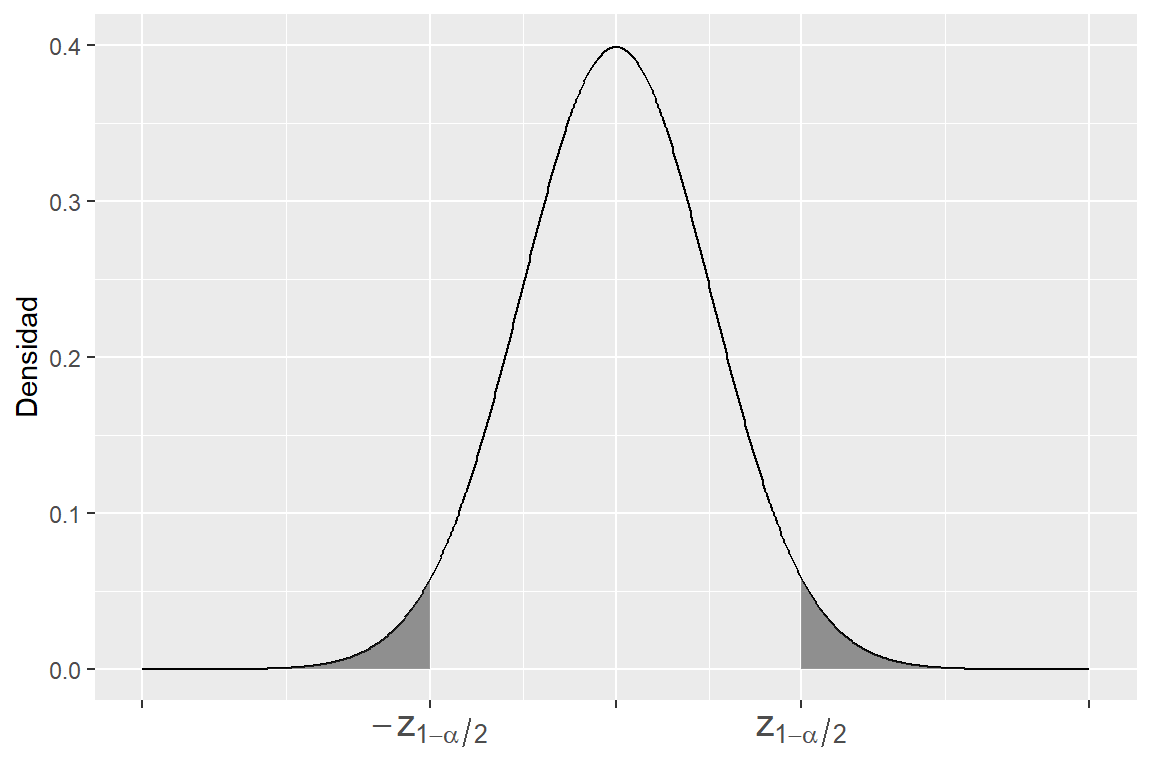
\includegraphics[width=0.7\textwidth]{Tema 4/figures/Figure 4}
\end{center}
La región $S_1$ está formada por los valores menores que $-z_{1-\frac{\alpha}{2} }$ o mayores que $z_{1-\frac{\alpha}{2} }$ .
\item Nos queda calcular, para nuestra muestra, el valor concreto del estadístico de prueba $z_0$:
    \begin{itemize}[label=\textrightarrow]
        \item Si pertenece a $S_1$, rechazaremos $H_0$ y afirmaremos $H_1$.
        \item Si no pertence a $S_1$, admitiremos $H_0$.
    \end{itemize}
\end{itemize}
\subsubsection*{Ejemplo}
\begin{tcolorbox}[colback=blue!5!white, colframe=blue!75!black, title=\textbf{En un proceso de producción}]
\begin{itemize}[label=\textbullet]
    \item La longitud de los artículos producidos se modeliza a través de una distribución Normal con media $\mu$.
    \item Por experiencia acerca del proceso, se cuantifica su desviación típica en $\sigma=1mm$.
    \item En condiciones de funcionamiento correcto, se espera que la longitud media de los artículos sea  $50$ mm.
    \item Para comprobar la calidad se decide tomar una muestra de 10 artículos que resultan tener la longitud media  $\overline{x}$ igual a 51 mm.
    \item Basándonos en esta muestra, ¿qué podemos decir acerca del funcionamiento del proceso?
\end{itemize}
\end{tcolorbox}
\subsection{Procedimiento, hipótesis unilateral}
Todo igual, excepto $S_1$.
\begin{itemize}[label=\textbullet]
    \item Si la hipótesis es $H_1:\mu>\mu_0$, la región de rechazo será
        \begin{center}
            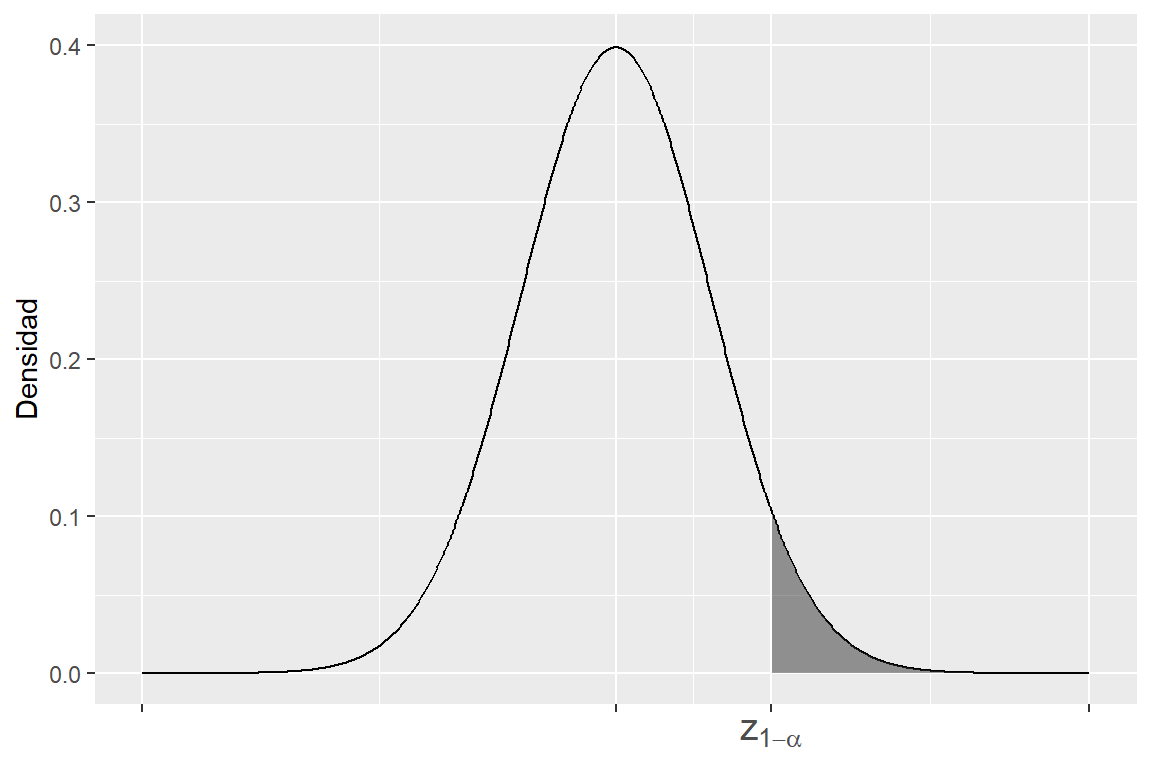
\includegraphics[width=0.7\textwidth]{Tema 4/figures/Figure 5}
        \end{center}
    \item Si la hipótesis es $H_1:\mu<\mu_0$, la región de rechazo será
        \begin{center}
            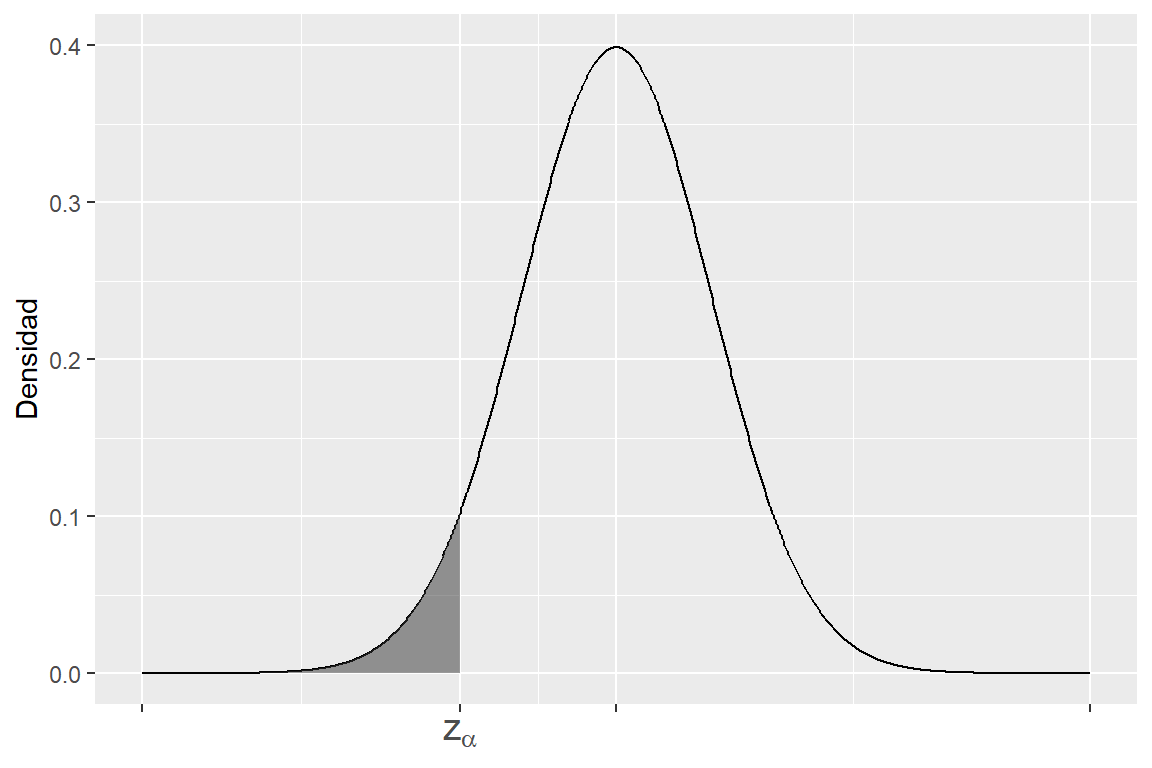
\includegraphics[width=0.7\textwidth]{Tema 4/figures/Figure 6}
        \end{center}
\end{itemize}
\subsection{El p-valor}
\begin{tcolorbox}[colback=blue!5!white, colframe=blue!75!black, title=\textbf{Definición}]
Consideramos un contraste, un test, y hemos observado una muestra concreta $\mathbf{x}$.
\begin{itemize}[label=\textbullet]
    \item El \lb{p-valor} es el nivel de significación más pequeño que nos lleve, para esa muestra $\mathbf{x}$, a rechazar la hipótesis nula.
    \item El p-valor está asociado a la región $S_1$ más pequeñas que nos lleve, para esa muestra, a rechazar $H_0$.
\end{itemize}
\end{tcolorbox}
\begin{tcolorbox}[colback=blue!5!white, colframe=blue!75!black, title=\textbf{Ejemplo}]
Volvamos al ejemplo de la longitud de los artículos producido. Para el contraste \[
    \begin{array}{l}
H_0:\mu=50,\\
        H_1:\mu\neq 50.
    \end{array}
\] Supongamos que hemos encontrado un estadístico de prueba $z_0=1.75$ y rechazamos $H_0$ al 95\% de confianza.

¿Cuál habría sido nuestra decisión al 90\%? ¿Y al 99\% de confianza?
\end{tcolorbox}
\begin{tcolorbox}[colback=olive!5!white, colframe=olive!75!black, title=\textbf{Importante}]
\begin{itemize}[label=\textbullet]
    \item Si rechazamos $H_0$ a un nivel de confianza dado, también la rechazamos a cualquier nivel de confianza menor.
    \item Para saber si la rechazamos a un nivel de confianza mayor, hay que probar.
\end{itemize}
\end{tcolorbox}
\begin{tcolorbox}[colback=blue!5!white, colframe=blue!75!black, title=\textbf{Para calcularlo:}]
\begin{itemize}[label=\textbullet]
    \item Dibujamos la densidad de la distribución muestral del estadístico de prueba.
    \item Colocamos el valor de $z_0$ calculado para mi muestra concreta.
    \item Dibujamos una región de rechazo de manera que $z_0$ coincida con una de las fronteras.
    \item El p-valor $\alpha_0$ es el valor de $\alpha$ correspondiente a esta región de rechazo.
\end{itemize}
\end{tcolorbox}
Para el ejemplo de las longitudes, sabemos $z_0=1.75$, lo colocamos:
\begin{center}
    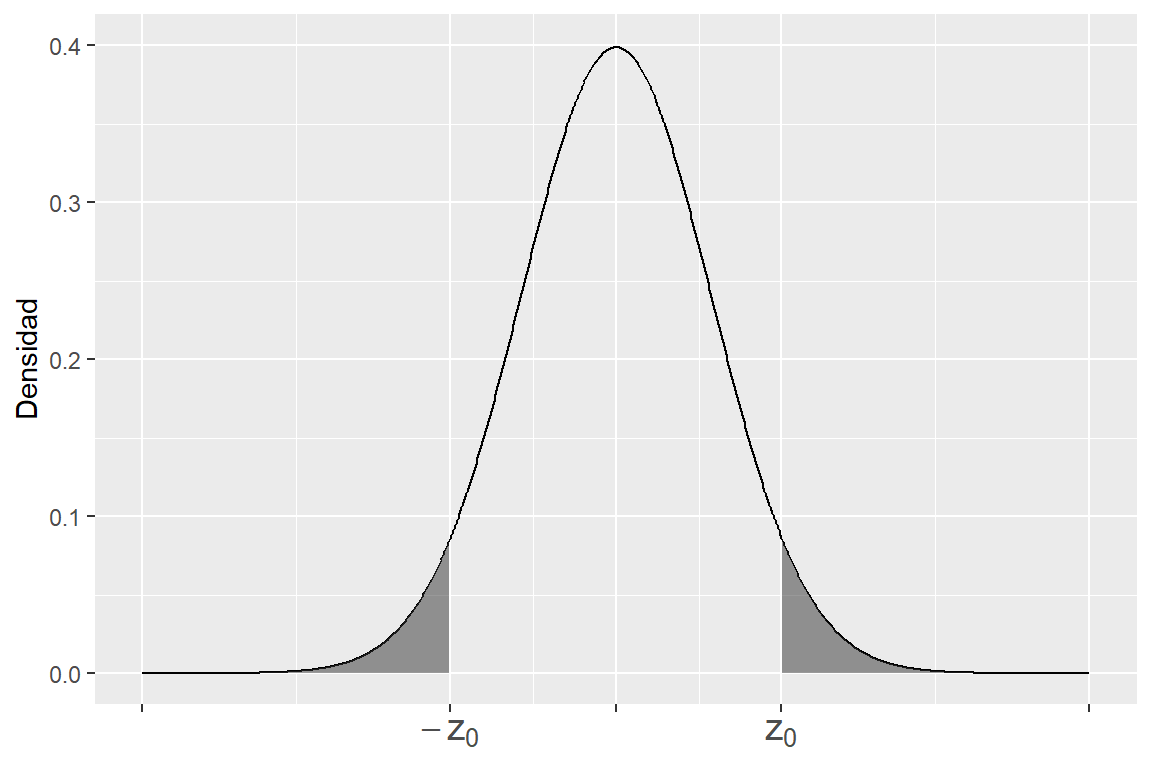
\includegraphics[width=0.7\textwidth]{Tema 4/figures/Figure 7}
\end{center}
Por lo que $\dfrac{\alpha_0}{2}=\mathbb{P}(Z\ge 1.75)$, es decir que $\alpha_0=2(1-\phi(1.75))$, lo que lleva a $\alpha_0\simeq 0.08$.
\begin{tcolorbox}[colback=olive!5!white, colframe=olive!75!black, title=\textbf{Para nuestro ejemplo}]
\begin{itemize}[label=\textbullet]
    \item Encontramos un  p-valor igual a 0.08, por lo que deducimos que la confianza máxima con la que podríamos haber rechazado $H_0$ es del 92\%.
    \item Deducimos que habríamos en particular rechazado $H_0$ al 90\% de confianza, pero, por ejemplo, no al 95\% de confianza.
\end{itemize}
\end{tcolorbox}
\begin{tcolorbox}[colback=olive!5!white, colframe=olive!75!black, title=\textbf{Cuidado con la interpretaión del p-valor}]
El p-valor se puede interpretar como una medida de compatibilidad de los datos con la hipótesis nula.
\begin{itemize}[label=\textbullet]
    \item No debemos usarlo como el único criterio para basar nuestra decisión.
    \item Es bueno hacer gráficas, considerar el contexto, ver si el efecto es relevante y no solamente significativo.
    \item Se debe evitar considerar $p-valor<0.05$ como un valor mágico que es sinónimo de efecto significativo.
\end{itemize}
\end{tcolorbox}
\subsection{Test óptimo}
\begin{tcolorbox}[colback=blue!5!white, colframe=blue!75!black, title=\textbf{Empezamos por considerar los tests con probabilidad de error tipo I menor o igual que $\alpha$:}]
\begin{itemize}[label=\textbullet]
    \item Dado $\alpha$, sea \[
    T_\alpha=\{\delta\in T|P_{i,\delta}(\theta)\le \alpha \text{ para todo }\theta\in \Theta_0\},
    \] llamaremos $\alpha$ el \lb{nivel de significación del test}.
\item Para un test $\delta$, se llama  \lb{tamaño} o \lb{extensión} de $\lambda$ a:  $\sup_{\theta\in \Theta_0}P_{I,\delta}(\theta)$.  
\end{itemize}
\end{tcolorbox}
\begin{tcolorbox}[colback=blue!5!white, colframe=blue!75!black, title=\textbf{Definición}]
Dado $\delta^*\in T_\alpha$ decimos que es \lb{óptimo} si \[
P_{II,\delta^*}(\theta)\le P_{II,\delta}(\theta)\text{ para todo $\delta\in T_\alpha$ y para todo $\theta\in \Theta_1$.}
\]  
\end{tcolorbox}
\subsection{Potencia de un test}
\begin{tcolorbox}[colback=blue!5!white, colframe=blue!75!black, title=\textbf{Definición}]
La \lb{función potencia}  de un test $\delta$ asocia a cada  $\theta$ la probabilidad de rechazar la hipótesis nula:  \[
\theta\mapsto \pi_\delta(\theta)=P_\theta(X \in S_1),\quad \text{con $\theta\in \Theta$}.
\] 
\end{tcolorbox}
\begin{tcolorbox}[colback=olive!5!white, colframe=olive!75!black, title=\textbf{Relación de la potencia con los errores}]
\begin{itemize}[label=\textbullet]
    \item Si $\theta\in \Theta_0$ entonces $\pi_\delta(\theta)=P_{I,\delta}(\theta)$.
    \item Si $\theta\in \Theta_1$ entonces \[
    \pi_\delta(\theta)=P_\theta(X\in S_1)=1-P_\theta(X\in S_0)=1-P_{II,\delta}(\theta).
    \] 
\end{itemize}
\end{tcolorbox}
\subsection{Test óptimo como el de máxima potencia}

Sea $\delta^*\in T_\alpha$, diremos que es el \lb{test uniforme de máxima potencia} para el contraste \[
H_0:\theta\in \Theta
\] frente a \[
H_1:\theta\in \Theta_1
\] si se verifica \[
\pi_{\delta^*})\theta\ge \pi_{\delta}(\theta)\text{ para todo $\delta\in T_\alpha$ y para todo $\theta\in \Theta_1$.}
\] 
\subsection{Procedimientos basados en la verosimilitud}
\begin{tcolorbox}[colback=olive!5!white, colframe=olive!75!black, title=\textbf{Un procedimiento natural}]
Puesto que la verosimilitud expresa la compatibilidad de los datos con el modelo considerado, es natural construir un test basado en la comparación de la verosimilitud para los valores de $\Theta_0$ y para los valores de $\Theta_1$.
\end{tcolorbox}
\begin{tcolorbox}[colback=olive!5!white, colframe=olive!75!black, title=\textbf{Constrastes de hipótesis simples}]
En este tipo de contraste los subconjunto del espacio paramétrico solo tienen un elemento, es decir $\Theta_0=\{\theta_0\} $ y $\Theta_1=\{\theta_1\} $ y por lo tanto los errores de ambos tipos son cantidades fijas. Implícitamente, estamos asumiendo que el parámetro es unidimensional.
\end{tcolorbox}
\subsection{Constrastes de hipótesis simples}
\begin{tcolorbox}[colback=blue!5!white, colframe=blue!75!black, title=\textbf{Lema de Neyman-Pearson}]
Sea $X\sim F(x,\theta),\Theta=\{\theta_0,\theta_1\},\mathbf{X}=(X_1,X_2,\dots,X_n) $, una muestra aleatoria simple de la población $X$,  $\alpha$ fijo con $0<\alpha<1$. Para contrastar la hipótesis nula $H_0:\theta=\theta_0$ frente a la hipótesis alternativa $H_1:\theta=\theta_1$, el test de región de rechazo: \[
S_1=\left\{ \mathbf{x}\in \mathrm{Sop}(\mathbf{X})\bigg|\dfrac{L(\mathbf{x},\theta_1)}{L(\mathbf{x},\theta_0)}\ge k \right\} 
\] con $k>0$, que además tenga tamaño  $\alpha$, es decir $\alpha=P(\mathbf{X}\in S_1|\theta=\theta_0)$, cumple que es el test de máxima potencia en la clase de los tests $T_\alpha$.
\end{tcolorbox}
\begin{itemize}[label=\color{red}\textbullet, leftmargin=*]
    \item \lb{Observaciones}
        \begin{itemize}[label=\textbullet]
            \item Si la distribución es de tipo continuo siempre se cumple que el test alcanza el tamaño obteniéndose el test de extensión de $\alpha$.
            \item Si la distribución es de tipo discreto, en general, el test de máxima potencia será de extensión menor que $\alpha$.
        \end{itemize}
    \item \lb{Demostración} 

        Sea $\delta^*$ el test definido anteriormente.
         \begin{itemize}[label=\textbullet]
            \item La condición \[
            \alpha=P(\mathbf{X}\in S_1|\theta=\theta_0)
            \] nos asegura que $\delta^*\in T_\alpha$. Sea ahora $\delta\in T_\alpha$ cualquiera. Tenemos que probar que: \[
            \pi_{\delta^*}(\theta_1)\ge \pi_{\delta}(\theta_1)
            \] supondremos $X$ variable aleatoria continua (en el caso discreto se razonará de forma análoga).
        \item Sea  $\mathbf{X}\in \mathrm{sop}(X)$ se verifica que: \[
                (\delta^*(\mathbf{X})-\delta(\mathbf{X}))(L(\mathbf{x},\theta_1)-kL(\mathbf{x},\theta_0))\ge 0.
        \] 
    \item Si $\delta(\mathbf{X})^*=1$ entonces: \[
    \dfrac{L(\mathbf{x},\theta_1)}{L(\mathbf{x},\theta_0)}\ge k\longleftrightarrow L(\mathbf{x},\theta_1)-kL(\mathbf{x},\theta_0)\ge 0
    \] y $\delta^*(\mathbf{X})-\delta(\mathbf{X})\ge 0$ ($\delta(\mathbf{X})$ sólo puede ser 0 o 1) y el producto es no negativo.
\item Si $\delta(\mathbf{X})^*=0$ entonces: \[
    \dfrac{L(\mathbf{x},\theta_1)}{L(\mathbf{x},\theta_0)}< k\longleftrightarrow L(\mathbf{x},\theta_1)-kL(\mathbf{x},\theta_0)< 0
\] y $\delta^*(\mathbf{X})-\delta(\mathbf{X})\le 0$ ($\delta(\mathbf{X})$ sólo puede ser 0 o 1) y el producto es no negativo.
\item La integral de la expresión anterior sobre el $\mathrm{sop}(\mathbf{X})$ será no negativa: \[
        \begin{array}{c}
\int_{\mathrm{sop}(\mathbf{X})}(\delta^*(\mathbf{X})-\delta(\mathbf{X}))(L(\mathbf{x},\theta_1)-kL(\mathbf{x},\theta_0))\mathrm{d}\mathbf{x}\ge 0\\ \int_{\mathrm{sop}(\mathbf{X})}\delta^*(\mathbf{X})L(\mathbf{x},\theta_1)\mathrm{d}\mathbf{x}-\int_{\mathrm{sop}(\mathbf{X})}\delta(\mathbf{X})L(\mathbf{x},\theta_1)\mathrm{d}\mathbf{x}-k\int_{\mathrm{sop}(\mathbf{X})}\delta^*(\mathbf{X})L(\mathbf{x},\theta_0)\mathrm{d}\mathbf{x}-\int_{\mathrm{sop}(\mathbf{X})}\delta(\mathbf{X})L(\mathbf{x},\theta_0)\mathrm{d}\mathbf{x}\ge 0
        \end{array}
\] 
notar que ambos contrastes solo toman el valor 1 en sus respectivas regiones de rechazo (y cero en las regiones de aceptación) con lo que al desarrollar los terminos de la integral tenemos: \[
\pi_{\delta^*}-\pi_\delta(\theta_1)-k(\pi_{\delta^*}(\theta_0)-\pi_\delta(\theta_0))\ge 0.
\]
\item Como $\delta\in T_\alpha$ tenemos que $\pi_\delta(\theta_0)\le \alpha$ con lo que: \[
0\le \alpha-\pi_\delta(\theta_0)=\pi_{\delta^*}(\theta_0)-\pi_\delta(\theta_0)
\] y por lo tanto: \[
k(\pi_{\delta^*}(\theta_0)-\pi_\delta(\theta_0))\ge 0
\] con lo que: \[
0\le \pi_{\delta^*}(\theta_1)-\pi_\delta(\theta_1)-k(\pi_{\delta^*}(\delta_0)-\pi_\delta(\theta_0))\le \pi_{\delta^*}(\theta_1)-\pi_\delta(\theta_1)
\] de donde se deduce: \[
\pi_{\delta^*}(\theta_1)\ge \pi_\delta(\theta_1)
\] que era lo que queríamos probar.
        \end{itemize}
\end{itemize}
\subsection{Hipótesis compuestas}
\begin{tcolorbox}[colback=olive!5!white, colframe=olive!75!black, title=\textbf{Planteamiento}]
En las aplicaciones a problemas reales no suelen plantearse, en general, contrastes de hipótesis simple y alternativa simple, pues las hipótesis alternativas no suelen ser tan precisas para que estén definidas por un único valor del parámetro. Consideremos ahora contrastes de hipótesis donde al menos una de ellas es compuesta.
\end{tcolorbox}
\begin{tcolorbox}[colback=blue!5!white, colframe=blue!75!black, title=\textbf{Casos}]
\begin{center}
    \begin{varwidth}{0.5\textwidth}
    \begin{multicols}{2}
   \begin{enumerate}[label=\alph*)]
       \item $\begin{array}{l}
           H_0:\theta=\theta_0\\
           H_1:\theta>\theta_0
       \end{array}$
       \item $\begin{array}{l}
           H_0:\theta=\theta_0\\
           H_1:\theta<\theta_0
       \end{array}$
       \item $\begin{array}{l}
           H_0:\theta\le \theta_0\\
           H_1:\theta>\theta_0
       \end{array}$
       \item $\begin{array}{l}
           H_0:\theta\ge \theta_0\\
           H_1:\theta<\theta_0
       \end{array}$
       \item $\begin{array}{l}
           H_0:\theta=\theta_0\\
           H_1:\theta\neq \theta_0
       \end{array}$
       \item $\begin{array}{l}
               H_0:\theta\in [\theta_1,\theta_2]\\
               H_1:\theta\notin [\theta_1,\theta_2]
       \end{array}$
   \end{enumerate} 
\end{multicols}
\end{varwidth}
\end{center}
En los casos a)-d) anteriores es posible obtener tests uniformes de máxima potencia para casos en los que la variable pertenece a la familia exponencial uniparamétrica.
\end{tcolorbox}
\subsection{Cociente de verosimilitudes monótono}
\begin{tcolorbox}[colback=blue!5!white, colframe=blue!75!black, title=\textbf{Resultado}]
Sea $X\sim F(x,\theta),\theta\in \Theta\subset\R$ y $X_1,\dots,X_n$ una muestra aleatoria simple de $X$. Decimos que  $X$ o  $F$ tienen la propiedad de cociente de verosimilitud monótono en el estadístico  $R=R(X_1,\dots,X_n)$, si para todo $\theta_0,\theta_1\in \Theta$ con $\theta_0<\theta_1$ se verifica que el cociente de verosimilitudes $\dfrac{L(\mathbf{x},\theta_1)}{L(\mathbf{x},\theta)}$, es una función monótona creciente de $R(\mathbf{x})$.
\end{tcolorbox}
\begin{tcolorbox}[colback=red!5!white, colframe=red!75!black, title=\textbf{Nota}]
A los efectos de la definición si $L(\mathbf{x},\theta_0)=0$ y $L(\mathbf{x},\theta_1)>0$, el cociente anterior se considerará igual a infinito.
\end{tcolorbox}
\begin{tcolorbox}[colback=blue!5!white, colframe=blue!75!black, title=\textbf{Familia exponencia uniparamétrica}]
Se dice que la variable $X\sim F(x,\theta)$ pertenece a la familia exponencia uniparamétrica si su función de verosimilitud se puede escribir en la forma: \[
L(\mathbf{x},\theta)=\exp \{A(\theta)T(\mathbf{x})+B(\theta)+h(\mathbf{x})\}
\] para toda muestra $\mathbf{x}$.

Si $A(\theta)$ es monótona creciente (decreciente) en $\theta$, entonces  $X$ tiene cociente de verosimilitud monótono en el estadístico $T(X_1,\dots,X_n)(-T(X_1,\dots,X_n))$.
\end{tcolorbox}

\begin{tcolorbox}[colback=blue!5!white, colframe=blue!75!black, title=\textbf{Cociente de verosimilitudes monótono}]
Sea $X\sim F(x,\theta),\theta\in \Theta\subset \R$ y $X_1,\dots,X_n$ una m.a.s de $X$. Supongamos que  $X$ tiene cociente de verosimilitud monótono en el estadístico $R=R(X_1,\dots,X_n)$ para contrastar $H_0:\theta=\theta_0$ frente a $H_1:\theta>\theta_0$, se sigue que el test \[
\delta_1(\mathbf{x})=\begin{cases}
    0 & \text{si }R(\mathbf{x})<c\\
    1 & \text{si }R(\mathbf{x})\ge c
\end{cases}
\] que cumpla $P_{I,\delta_1}(\theta_0)=\alpha$, es el test uniforme de máxima potencia en la clase de tests $T_\alpha=\{\delta\in T|P_{I,\delta}(\theta_0)\le \alpha\} $, con $0<\alpha<1$.
\end{tcolorbox}
El teorema anterior se extiende al constrante $H_0:\theta\le \theta_0$ frente a $H_1:\theta>\theta_0$.
\begin{tcolorbox}[colback=blue!5!white, colframe=blue!75!black, title=\textbf{Cociente de verosimilitudes monótono}]
Sea $X\sim F(x,\theta),\theta\in \Theta\subset \R$ y $X_1,\dots,X_n$ una m.a.s de $X$. Supongamos que  $X$ tiene cociente de verosimilitud monótono en el estadístico $R=R(X_1,\dots,X_n)$ para contrastar $H_0:\theta=\theta_0$ frente a $H_1:\theta>\theta_0$, se sigue que el test \[
\delta_1(\mathbf{x})=\begin{cases}
    0 & \text{si }R(\mathbf{x})>c\\
    1 & \text{si }R(\mathbf{x})\le c
\end{cases}
\] que cumpla $P_{I,\delta_1}(\theta_0)=\alpha$, es el test uniforme de máxima potencia en la clase de tests $T_\alpha=\{\delta\in T|P_{I,\delta}(\theta_0)\le \alpha\} $, con $0<\alpha<1$.
\end{tcolorbox}
El teorema anterior se extiende al constrante $H_0:\theta\ge \theta_0$ frente a $H_1:\theta<\theta_0$.
\subsection{Constrastes de hipótesis compuesta}
La metodología anterior no se puede aplicar a los casos e) y f) y en los casos de parámetros que no sean unidimensionales. Por tanto, es importante para muchos problemas prácticos, disponer de métodos de construcción de constrastes, basados en principios razonables y que permitan diseñar el test según el problema planteado. El método más importante lo constituye el \textbf{test de la razón de verosimilitudes generalizado}. 
\begin{tcolorbox}[colback=blue!5!white, colframe=blue!75!black, title=\textbf{Razón de verosimilitudes Generalizada (RVG)}]
Se llama razón de verosimilitudes generalizada para constrastar la hipótesis $H_0:\theta\in \Theta$ frente $H_1:\theta\in\Theta_1$ al cociente \[
\lambda(\mathbf{x})=\dfrac{\displaystyle \sup_{\theta\in \Theta_0}L(\mathbf{x};\theta)}{\displaystyle \sup_{\theta\in\Theta_1}L(\mathbf{x};\theta)}.
\] 
\end{tcolorbox}
\subsection{Procedimiento basado en la verosimilitud}
\begin{tcolorbox}[colback=blue!5!white, colframe=blue!75!black, title=\textbf{Test de razón de verosimilitud generalizada}]
Un test de razón de verosimilitud generalizada (RVG) para las hipótesis anteriores es aquel que tiene región crítica de la forma \[
S_1=\left\{ \mathbf{x}\in \mathrm{Sop}(X_1,\dots,X_n)|\lambda(\mathbf{x})=\dfrac{\displaystyle \sup_{\theta\in \Theta_0}L(\mathbf{x};\theta)}{\displaystyle \sup_{\theta\in \Theta}L(\mathbf{x};\theta)}<k \right\} 
\] 
Determinamos la constante $k$, imponiendo que el test tenga extensión $\alpha$, es decir: \[
\sup_{\theta\in\Theta_0}P((X_1,\dots,X_n)\in S_1|\theta)=\alpha.
\] 
\end{tcolorbox}
\subsection{Test RVG para la media de una población normal con varianza conocida}
\begin{tcolorbox}[colback=blue!5!white, colframe=blue!75!black, title=\textbf{Ejercicio}]
\begin{itemize}[label=\textbullet]
    \item $X\sim \mathcal{N}(\mu,\sigma^2)$, suponemos $\sigma$ conocida.
    \item M.a.s  $X_1,\dots,X_n$ de $X$.
    \item Formulamos las hipótesis  \[
            \begin{array}{l}
    H_0:\mu=\mu_0\\
    H_1:\mu\neq \mu_0
            \end{array}
    \] 
\end{itemize}
\begin{enumerate}[label=\arabic*)]
    \item Demostrar que el test que rechaza $H_0$ si $\left| \dfrac{\mathbf{\overline{X}}-\mu_0}{\sigma / \sqrt{n} } \right| >z_{1-\frac{\alpha}{2} }$ es de extensión $\alpha$.
    \item Demostrar que el test anterior es el test de RVG.
\end{enumerate}
\end{tcolorbox}
\textbf{¿Es de extensión $\alpha$?} 
\begin{itemize}[label=\textbullet]
    \item Hemos de comrpboar que: $\sup_{\theta\in \Theta_0}P_{i,\delta}(\theta)=\alpha$.
    \item En este caso $H_0$ es simple, si $\mu=\mu_0$ se cumple que $\dfrac{\mathbf{\overline{X}}-\mu_0}{\sigma / \sqrt{n} }\sim \mathcal{N}(0,1)$. \[
    P\left( \left| \dfrac{\mathbf{\overline{X}}-\mu_0}{\sigma / \sqrt{n} } \right|>z_{1-\frac{\alpha}{2} }|\mu_0  \right) =\alpha.
    \] 
    \begin{center}
        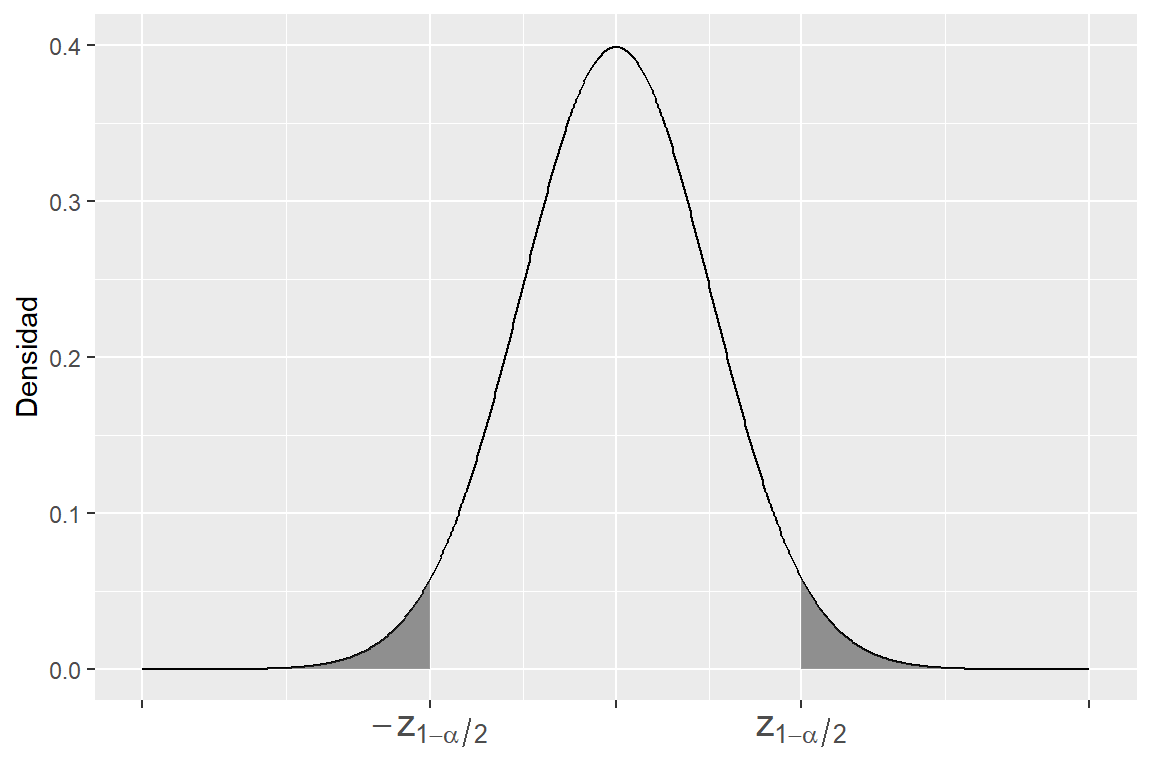
\includegraphics[width=0.7\textwidth]{Tema 4/figures/Figure 4}
    \end{center}
\end{itemize}
\textbf{¿Es el test de RVG?}
\[
\lambda(\mathbf{x})=\dfrac{\displaystyle \sup_{\mu=\mu_0}L(\mathbf{x};\mu)}{\displaystyle \sup_{\mu\in R}L(\mathbf{x};\mu)}.
\] 
\begin{itemize}[label=\textbullet]
    \item Numerador: \[
    L(\mathbf{X};\mu_0)=\dfrac{1}{\sigma^{\frac{n}{2} }(2\pi)^{\frac{n}{2} }}\exp\left( -\dfrac{1}{2\sigma^2}\sum_{i=1}^{n} (x_i-\mu_0)^2 \right) 
    \] 
\item El supremos en el denominador se alcanza en el EMV $\hat{\mu}=\overline{x}_n$.

    \[
        \lambda(\mathbf{x})=\exp\left( -\dfrac{n}{2\sigma^2}\sum_{i=1}^{n} (\overline{x}_n-\mu_0)^2 \right)
    \] 
\end{itemize}
\textbf{¿Es el test de RVG?} 
\begin{itemize}[label=\textbullet]
    \item Determinamos la constante $k$, imponiendo que el test tenga extensión  $\alpha$, es decir, \[
    \begin{array}{c}
        P(\lambda(\mathbf{x})<k|\mu_0)=\alpha\\
        \begin{aligned}
            \alpha&= P\left( 0<\exp\left( -\dfrac{n}{2\sigma^2}\sum_{i=1}^{n} (\overline{x}_n-\mu_0)^2 \right) <k|\mu_0 \right)  \\
            &= P\left( -\infty<-\dfrac{n}{2\sigma^2}\sum_{i=1}^{n} (\overline{x}_n-\mu_0)^2<\log(k)|\mu_0 \right)  \\
            &= P\left( \left( \dfrac{\overline{x}_n-\mu_0}{\sigma / \sqrt{n} } \right) ^2>-2\log(k)|\mu_0 \right)  \\
            &= P\left( \left| \dfrac{\overline{x}_n-\mu_0}{\sigma / \sqrt{n} } \right| >\sqrt{-2\log(k)}|\mu_0  \right)=P\left( \left| \dfrac{\overline{x}_n-\mu_0}{\sigma /\sqrt{n} } \right| >c|\mu_0 \right)   \\
        \end{aligned}
    \end{array}
    \] tomamos $c\impliedby_{1-\frac{\alpha}{2} }$.
\end{itemize}
\subsection{Test de razón de verosimilitudes generalizada}
\begin{tcolorbox}[colback=olive!5!white, colframe=olive!75!black, title=\textbf{Lo más difícil}]
Aunque el test RVG sea un test que suele tener buenas propiedades en cuanto a errores, para muchos modelos, no es sencillo deducir su distribución muestral.
\end{tcolorbox}
\begin{tcolorbox}[colback=blue!5!white, colframe=blue!75!black, title=\textbf{Aproximación asintótica de la distribución muestral para el test RVG}]
Para el contraste \[
H_0:\theta\in \Theta_0
\] frente a la alternativa \[
H_1:\theta\in \Theta_1
\] si $\dim(\Theta)=q$ y  $\dim(\Theta_0)=q'$ se verifica, bajo ciertas condiciones, que el estadístico $-2\log\lambda(\mathbf{X})$ converge en distribución a una ji-cuadrado con $q-q'$ grados de libertad.
\end{tcolorbox}
\subsection{Test de bondad de ajuste}
\begin{tcolorbox}[colback=blue!5!white, colframe=blue!75!black, title=\textbf{Es un contraste no paramétrico}]
\begin{itemize}[label=\textbullet]
    \item Su objetivo es comprobar hasta qué punto los daots observados parecen haber sido generados por una distribución de probabilidad dada.
    \item Se conoce como "contraste chi-cuadrado", porque es la distribución que usamos para construir nuestra regla de decisión.
\end{itemize}
\end{tcolorbox}
\begin{tcolorbox}[colback=blue!5!white, colframe=blue!75!black, title=\textbf{Primer ejemplo, el caso más sencillo:}]
\begin{itemize}[label=\textbullet]
    \item Tenemos $k$ clases posibles asociadas a un experimento aleatorio: $A_1,\dots,A_k$.
    \item Tenemos unos valores esperados para sus probabilidades \[
    p_1=P(A_1),\dots,p_k=P(A_k).
    \] 
\item Observamos $n$ realizaciones del experimento y queremos decidir si lo observado es compatible con los valores esperados.
\end{itemize}
\end{tcolorbox}
\subsection*{Caso sencillo bondad de ajuste}
\begin{tcolorbox}[colback=blue!5!white, colframe=blue!75!black, title=\textbf{El caso más sencillo:}]
\begin{itemize}[label=\textbullet]
    \item Planteamos \[
    \begin{array}{l}
        H_0:P(A_i)=p_i,\,i=1,\dots,k\\
        H_1:\text{Existe $i$ tal que  $P(A_i)\neq p_i$.}
    \end{array}
    \] 
\item Tenemos $k$ clases posibles asociadas a un experimento aleatorio: $A_1,\dots,A_k$.
\item Tenemos unos valores esperados para sus probabilidades \[
p_1=P(A_1),\dots,p_k=P(A_k).
\] 
\item Observamos $n$ realizaciones del experimento y queremos decidir si lo observado es compatible con los valores esperados.
\end{itemize}
\end{tcolorbox}
\subsection*{Caso sencillo bondad de ajuste: grupo sanguíneo}
\begin{tcolorbox}[colback=blue!5!white, colframe=blue!75!black, title=\textbf{Cuatro grupos sanguíneos}]
Experimento: escoger una persona
\begin{itemize}[label=\textbullet]
    \item $A_1=\text{"Su grupo es O"},A_2=\text{"Su grupo es A"},A_3=\text{"Su grupo es B"},A_4=\text{"Su grupo es AB"}.$ 
    \item Los valores esperados para sus probabilidades son $$p_1=43\%,p_2=40\%,p_3=12\%,p_4=5\%.$$ 
    \item En un grupo de 250 personas, observamos $f_1=110\text{ "O", }f_2=100\text{"A"},f_3=30\text{"B"},f_4=10\text{"AB"}$.
    \item En el grupo de 250, esperamos $\hat{f_1}=250\times 43\%\simeq 107.5\text{"O"},\hat{f_2}=2500\times 40\%\simeq 100\text{"A"},\hat{f_3}=250\times 12\%\simeq 30\text{"B"},\hat{f_4}=250\times 5\%\simeq 12.5\text{"AB"}$.
    \item Escribimos los datos en una tabla 
        \begin{center}
            \begin{tabular}{p{2cm}llll}
                \textbf{Clases} & $A_1$ & $A_2$ & $A_3$ & $A_4$\\ \hline
                Frecuencia observada & $f_1=110$ & $f_2=100$ & $f_3=30$ & $f_4=10$\\ \hline
                Frecuencia esperada & $\hat{f_1}=107.5$ & $\hat{f_2}=100$ & $\hat{f_3}=30$ & $\hat{f_4}=12.5$
            \end{tabular}
        \end{center}
\end{itemize}
\end{tcolorbox}
\subsubsection*{Construimos el estadístico para el constraste:}
\begin{tcolorbox}[colback=blue!5!white, colframe=blue!75!black, title=\textbf{El estaístico chi-cuadrado de Pearson}]
Para constrastar \[
\begin{array}{l}
    H_0:P(A_i)=p_i,\:i=1,\dots,k\\
    H_1:\text{Existe $i$ tal que  $P(A_i)\neq p_i$.}
\end{array}
\] 
Karl Pearson propuso el estadístico \[
\chi^2=\sum_{i=1}^{k} \dfrac{\left( f_i-\hat{f_i} \right) ^2}{\hat{f_i}}.
\] 
Si $n$ es suficientemente grande,  \[
\chi^2=\sum_{i=1}^{k} \dfrac{\left( f_i-\hat{f_i} \right) ^2}{\hat{f_i}}\text{ es aprox. $\chi_{k-1}^2$. }
\] 
\end{tcolorbox}
\[
\chi^2=\sum_{i=1}^{k} \dfrac{\left( f_i-\hat{f_i} \right) ^2}{\hat{f_i}}=\dfrac{(100-107.5)^2}{107.5}+\dfrac{0^2}{100}+\dfrac{0^2}{30}+\dfrac{(10-12.5)^2}{12.5}=1.02
\] 
Para calcular el p-valor, lo comparamos con los cuantiles de una $\chi_3^2$, valores extremos positivos nos llevan a rechazar $H_0$.
\begin{tcolorbox}[colback=blue!5!white, colframe=blue!75!black, title=\textbf{p-valor:}]
Encontramos $p-\text{valor}=0.79$, lo que nos lleva a afirmar que los datos apoyan la hipótesis nula, y son compatibls con los valores esperados $p_1=43\%\text{"O"},p_2=40\%\text{"A"},p_3=12\%\text{"B"},p_4=5\%\text{"AB"}$.
\end{tcolorbox}
\begin{tcolorbox}[colback=olive!5!white, colframe=olive!75!black, title=\textbf{Validez de la aproximación de la distribución de estadístico de Pearson por un $\chi_{k-1}^2$.}]
$n$ debe ser "suficientemente" grande.
\begin{itemize}[label=\textbullet]
    \item Se suele considerar que todas las frecuencias esperadas deben ser al menos 5, excepto una, y que esa sea mayor que 0.5.
    \item Si dos de ellas son pequeñas, entonces esas no deben ser menor que 1, y el resto debe ser al menos 5.
    \item Si no se cumple, se agrupan clases.
\end{itemize}
\end{tcolorbox}
\subsubsection*{Segundo caso: debemos estimar parámetros para calcular las frecuencias esperadas.}
\begin{tcolorbox}[colback=blue!5!white, colframe=blue!75!black, title=\textbf{Segundo ejemplo, un caso común:}]
\begin{itemize}[label=\textbullet]
    \item Tenemos $k$ clases posibles asociadas a un experimento aleatorio $A_1,\dots,A_k$.
    \item Los valores esperados para las probabilidades $p_1=P(A_1),\dots,p_k=P(A_k)$ dependen de unos parámetros desconocidos.
    \item Observamos $n$ realizaciones del experimento y queremos decidir si lo observado es compatible con los valores esperados.
    \item Planteamos $H_0:P(A_i)=p_i,\: i=1,\dots,k$ frente a $H_1$: Existe $i$ tal que $P(A_i)\neq p_i$.
\end{itemize}
\end{tcolorbox}
\begin{tcolorbox}[colback=olive!5!white, colframe=olive!75!black, title=\textbf{Procederemos igual que antes, pero:}]
\begin{itemize}[label=\textbullet]
    \item Estimaremos los parámetros desconocidos a partir de las observaciones.
    \item El estadístico de Pearson tendrá como distribución aproximada $\chi_{k-d-1}^2$, donde $d$ es el número de parámetros que debemos estimar para aproximar las frecuencias esperadas.
\end{itemize}
\end{tcolorbox}
\subsubsection*{Ejemplo: daltonismo}
\begin{tcolorbox}[colback=blue!5!white, colframe=blue!75!black, title=\textbf{La incidencia del daltonismo depende del sexo:}]
\begin{itemize}[label=\textbullet]
    \item Los genes responsables del daltonismo se encuentran en el cromosoma $X$.
    \item Los hombres tienen un solo cromosoma  $X\Longrightarrow $ una copia del gen defectuoso en su cromosoma $X$ es suficiente para ser daltónico.
    \item Las mujeres tienen dos cromosomas  $X\Longrightarrow $ dos copias del gen defectuoso son necesarias para ser daltónicas.
\end{itemize}
\end{tcolorbox}
\begin{tcolorbox}[colback=blue!5!white, colframe=blue!75!black, title=\textbf{Si llamamos $q$ a la probabilidad de que el cromosoma  $X$ tenga el gen defectuoso y  $p=1-q$.}]
Tenemos:
\begin{center}
    \begin{tabular}{cll}
      & \textbf{Masculino} & \textbf{Femenino}\\ \hline
        Normales & $\dfrac{p}{2}$ & $\dfrac{p^2}{2}+pq$\\ \hline
        Daltónicos & $\dfrac{q}{2}$ & $\dfrac{q^2}{2}$
 \end{tabular}   
\end{center}
\end{tcolorbox}
\subsection*{Datos observados:}
\begin{tcolorbox}[colback=blue!5!white, colframe=blue!75!black, title=\textbf{Para una muestra de 1000 personas:}]
\begin{center}
    \begin{tabular}{cll}
        & \textbf{Masculino} & \textbf{Feminino} \\ \hline
        Normales & 442 & 514\\
        Daltónicos & 38 & 6\\
    \end{tabular}
\end{center}
\end{tcolorbox}
